Amostre o sinal  a um período de amostragem e determine os seguintes:

\subsubsection*{(a) \textbf{(1,0 pontos) }}
Calcule a DFT e FFT do sinal amostrado com uma janela de somente 32 amostras. É possível observar no espectro as senóides?

\begin{figure}[H]
    \centering
    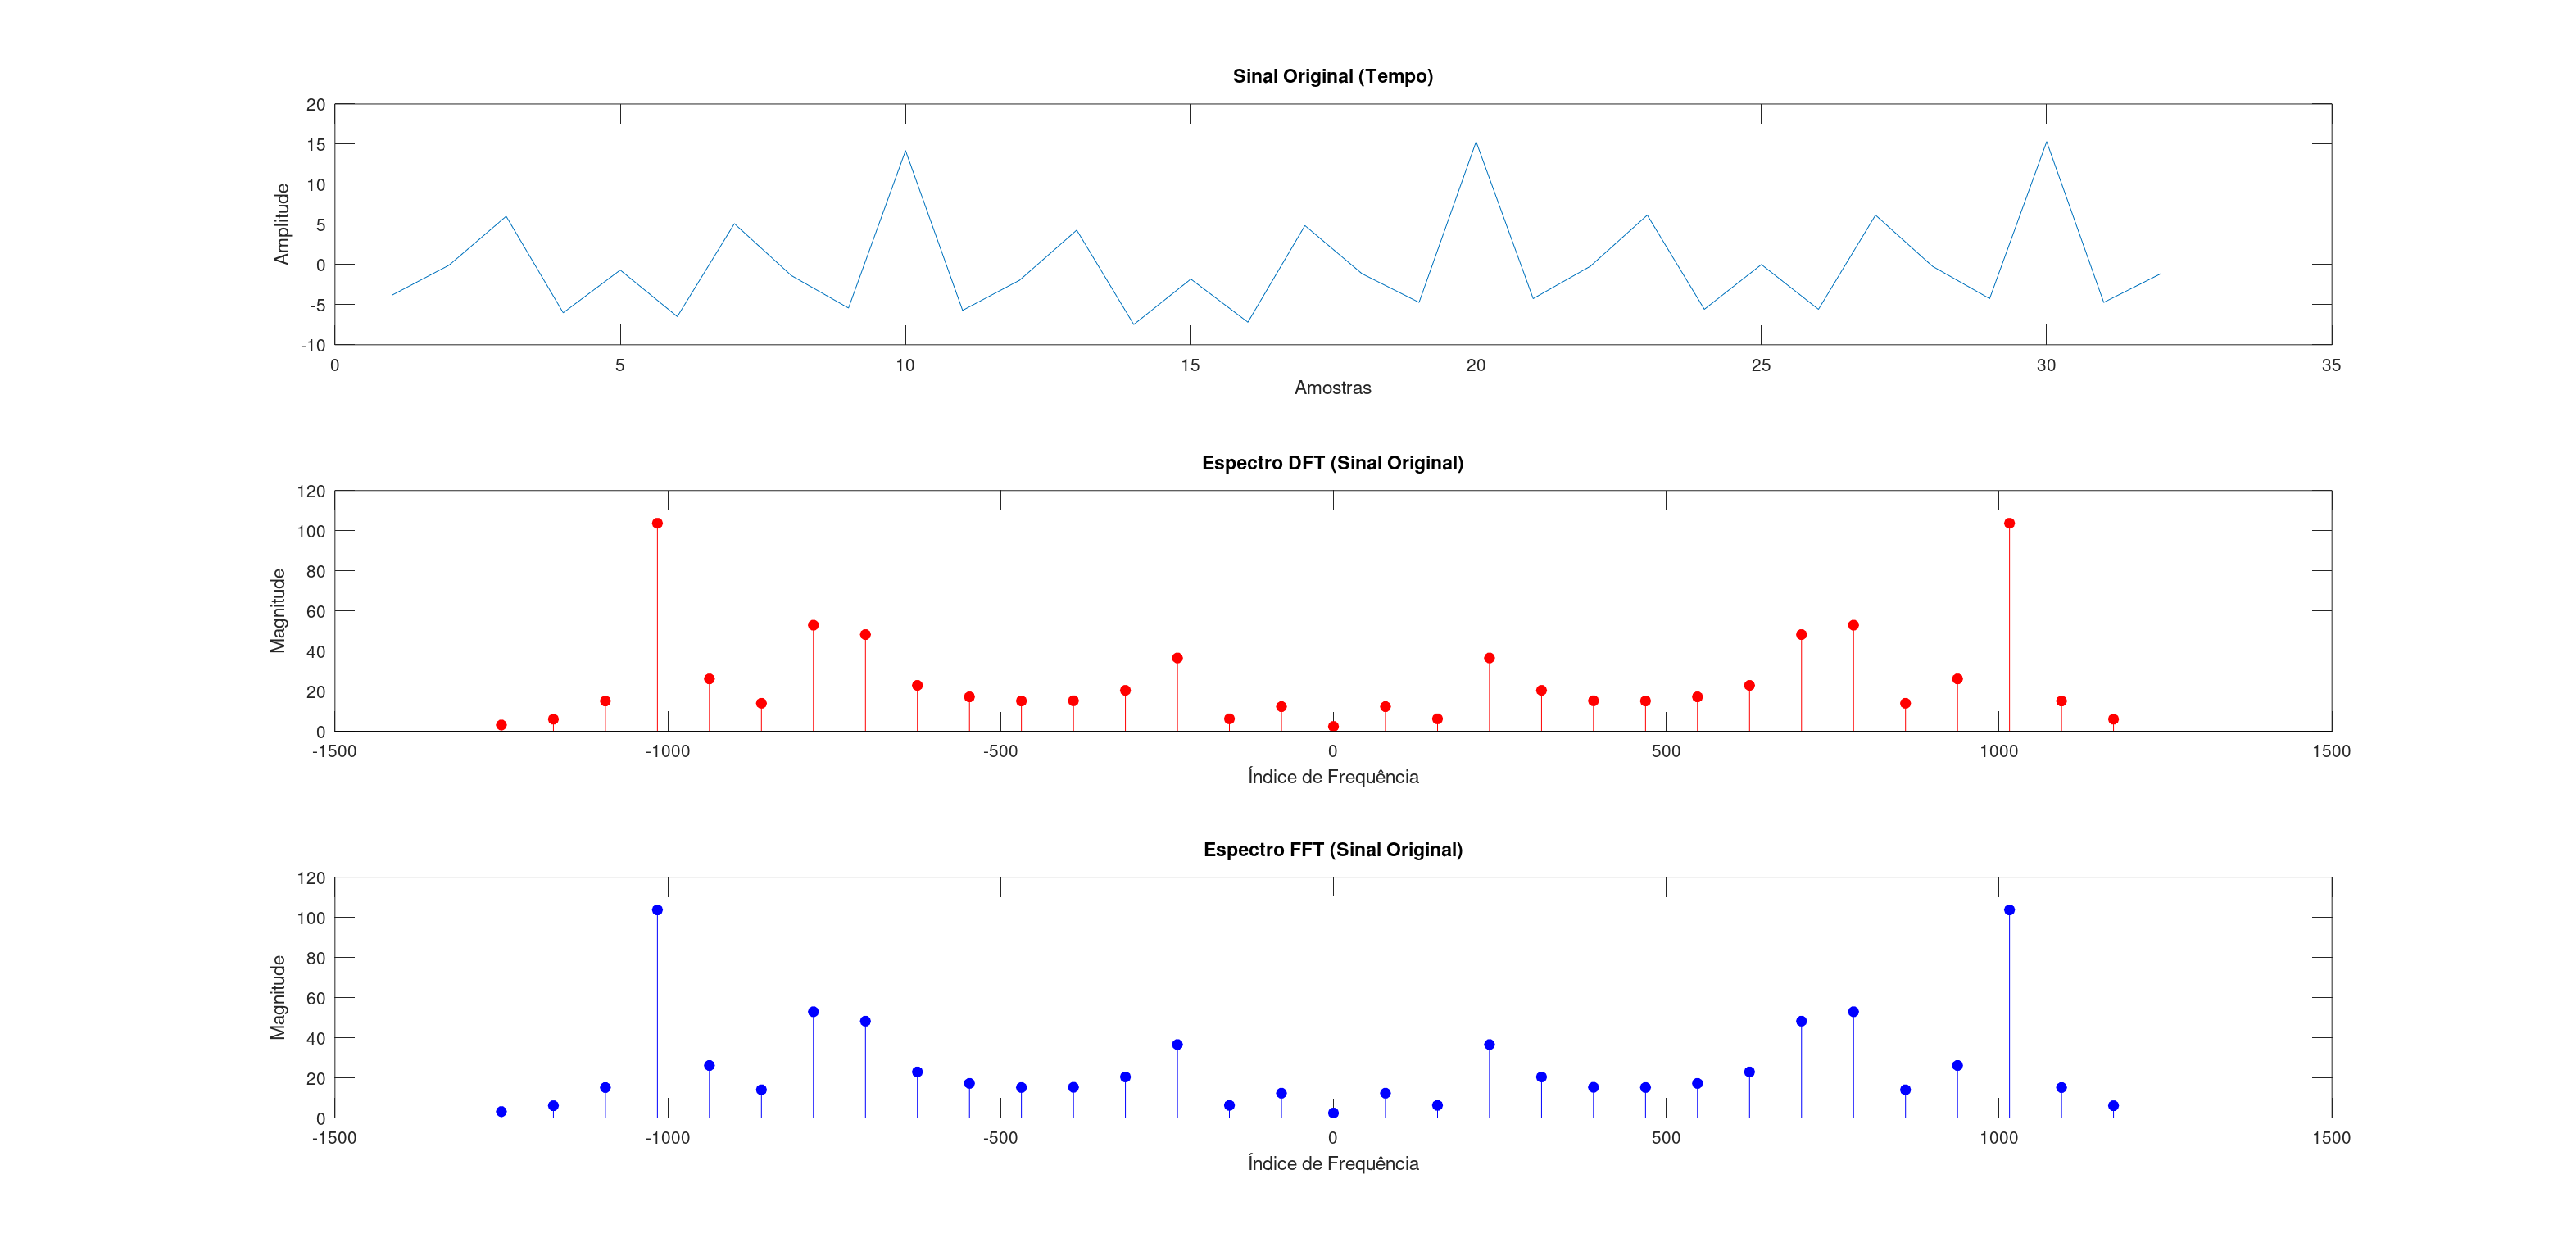
\includegraphics[width=1\linewidth]{03_experimental_analysis/plot_results/32_samples_dft_fft.png}
    \caption{DFT+FFT Aplicada a 32 amostras}
    \label{fig:signal_32samples_fft-dft}
\end{figure}

%%%%%%%%%%%%%%%%%%%%%%%%%%%%%%%%%%%%%%%%%%%%%%%%%%%%%%%%%%%%%%%%%%%%%%
\subsubsection*{(b) \textbf{(1,0 pontos)}}
Aumente o comprimento do item anterior para 64 amostras, aumentando 32 zeros à direita das amostras originais. Calcule a DFT e FFT. Compare com o item anterior e comente seus resultados.

\begin{figure}[H]
    \centering
    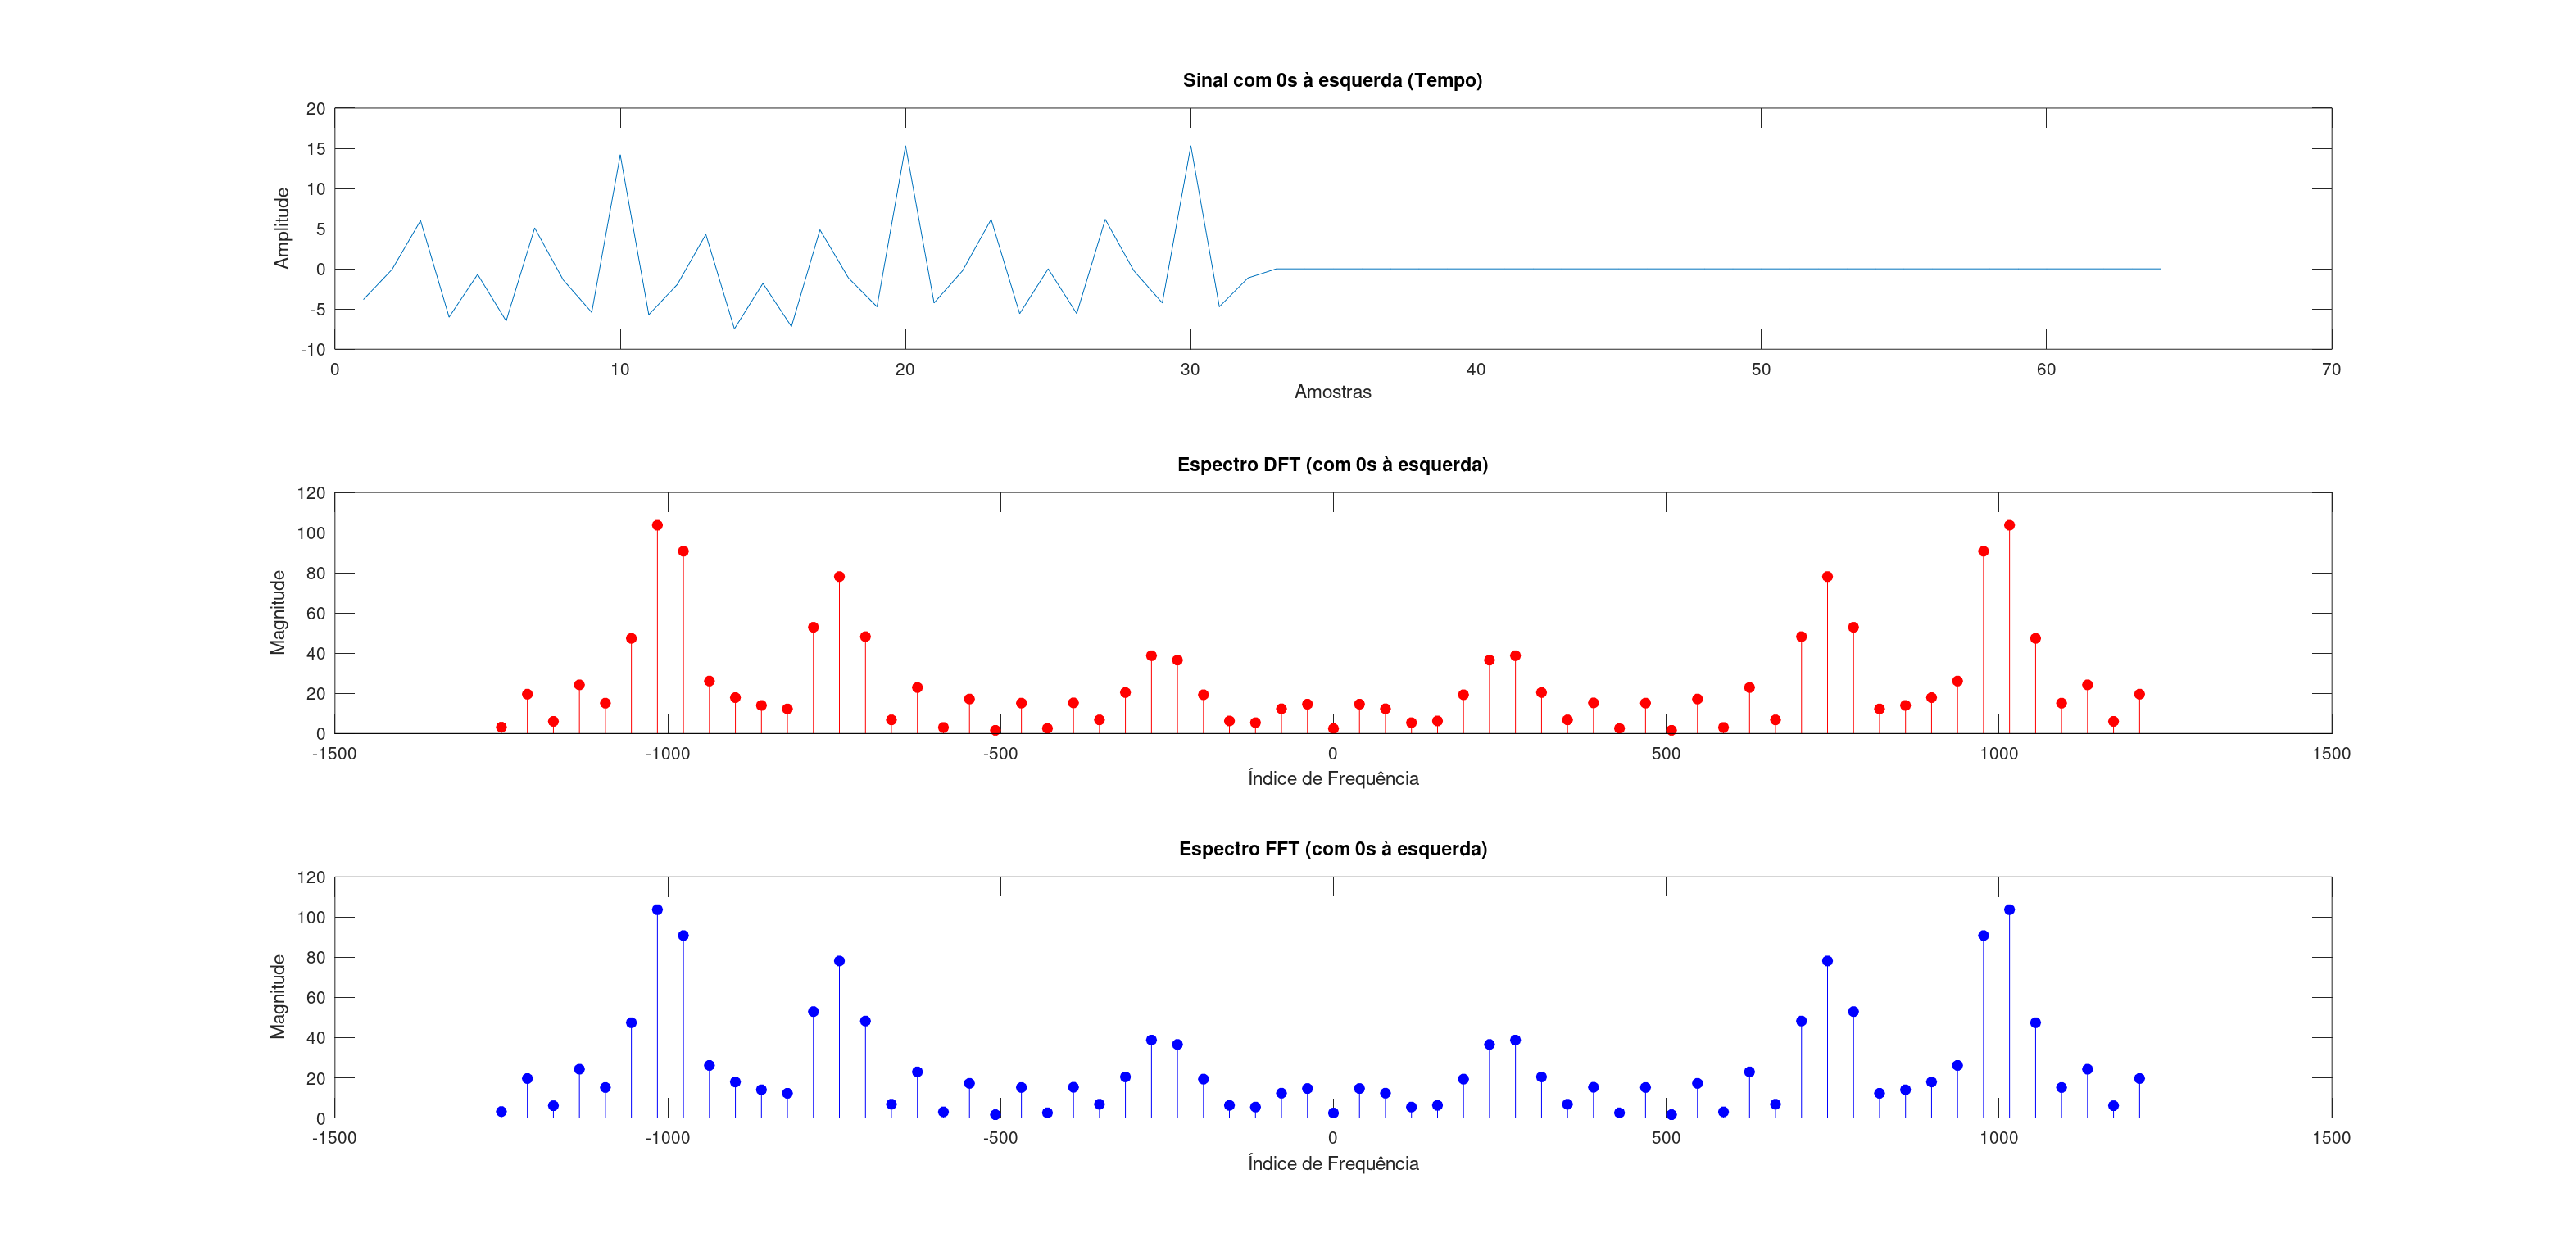
\includegraphics[width=1\linewidth]{03_experimental_analysis/plot_results/32_samples_dft_fft_padded.png}
    \caption{DFT+FFT Aplicada a 32 amostras com 32 zeros à direita}
    \label{fig:signal_32samples_fft-dft_padded}
\end{figure}

%%%%%%%%%%%%%%%%%%%%%%%%%%%%%%%%%%%%%%%%%%%%%%%%%%%%%%%%%%%%%%%%%%%%%%
\subsubsection*{(c) \textbf{(1,0 pontos)}}
Calcule a DFT e FFT usando uma janela de 64 amostras. É possivel observar no espectro as senóides?

%%%%%%%%%%%%%%%%%%%%%%%%%%%%%%%%%%%%%%%%%%%%%%%%%%%%%%%%%%%%%%%%%%%%%%
\subsubsection*{(d) \textbf{(1,0 pontos)}}
Aumente o comprimento do item anterior para 128 amostras, aumentando 64 zeros à direita das amostras originais. Calcule a DFT e FFT. Compare com o item anterior e comente seus resultados.

%%%%%%%%%%%%%%%%%%%%%%%%%%%%%%%%%%%%%%%%%%%%%%%%%%%%%%%%%%%%%%%%%%%%%%
\subsubsection*{(e) \textbf{(1,0 pontos)}}
E assim por diante, repita os ítens (a) e (b) para 256, 512 e 1024 amostras do sinal.

\subsubsection*{(f) \textbf{(1,0 pontos)}}
Monte numa tabela comparativa a quantidade de operações (produtos e somas) realizadas.

\begin{table}[ht]
    \centering
    \begin{tabular}{lccc}
    \textit{\textbf{Amostras}}            & \textbf{DFT (Ops)} & \textbf{FFT (Sums)} & \textbf{FFT (Mult)} \\
    \textit{32}                       & 1024                                & 160                  & 80                            \\
    \textit{32 + 32 0s}     & 4096                                & 384                  & 192                           \\
    \textit{64}                       & 4096                                & 384                  & 192                           \\
    \textit{64 + 64 0s}     & 16384                               & 896                  & 448                           \\
    \textit{128}                      & 16384                               & 896                  & 448                           \\
    \textit{128 + 128 0s}   & 65536                               & 2048                 & 1024                          \\
    \textit{256}                      & 65536                               & 2048                 & 1024                          \\
    \textit{256 + 256 0s}   & 262144                              & 4608                 & 2304                          \\
    \textit{512}                      & 262144                              & 4608                 & 2304                          \\
    \textit{512 + 512 0s}   & 1048576                             & 10240                & 5120                          \\
    \textit{1024}                     & 1048576                             & 10240                & 5120                          \\
    \textit{1024 + 1024 0s} & 4194304                             & 22528                & 11264                        
    \end{tabular}
    \caption{Comparativo da quantidade de operações (produtos e somas) realizadas em diferentes configurações de amostras.}
    \label{tab:operacoes_comparativo}
\end{table}

